\documentclass[1p]{elsarticle_modified}
%\bibliographystyle{elsarticle-num}

%\usepackage[colorlinks]{hyperref}
%\usepackage{abbrmath_seonhwa} %\Abb, \Ascr, \Acal ,\Abf, \Afrak
\usepackage{amsfonts}
\usepackage{amssymb}
\usepackage{amsmath}
\usepackage{amsthm}
\usepackage{scalefnt}
\usepackage{amsbsy}
\usepackage{kotex}
\usepackage{caption}
\usepackage{subfig}
\usepackage{color}
\usepackage{graphicx}
\usepackage{xcolor} %% white, black, red, green, blue, cyan, magenta, yellow
\usepackage{float}
\usepackage{setspace}
\usepackage{hyperref}

\usepackage{tikz}
\usetikzlibrary{arrows}

\usepackage{multirow}
\usepackage{array} % fixed length table
\usepackage{hhline}

%%%%%%%%%%%%%%%%%%%%%
\makeatletter
\renewcommand*\env@matrix[1][\arraystretch]{%
	\edef\arraystretch{#1}%
	\hskip -\arraycolsep
	\let\@ifnextchar\new@ifnextchar
	\array{*\c@MaxMatrixCols c}}
\makeatother %https://tex.stackexchange.com/questions/14071/how-can-i-increase-the-line-spacing-in-a-matrix
%%%%%%%%%%%%%%%

\usepackage[normalem]{ulem}

\newcommand{\msout}[1]{\ifmmode\text{\sout{\ensuremath{#1}}}\else\sout{#1}\fi}
%SOURCE: \msout is \stkout macro in https://tex.stackexchange.com/questions/20609/strikeout-in-math-mode

\newcommand{\cancel}[1]{
	\ifmmode
	{\color{red}\msout{#1}}
	\else
	{\color{red}\sout{#1}}
	\fi
}

\newcommand{\add}[1]{
	{\color{blue}\uwave{#1}}
}

\newcommand{\replace}[2]{
	\ifmmode
	{\color{red}\msout{#1}}{\color{blue}\uwave{#2}}
	\else
	{\color{red}\sout{#1}}{\color{blue}\uwave{#2}}
	\fi
}

\newcommand{\Sol}{\mathcal{S}} %segment
\newcommand{\D}{D} %diagram
\newcommand{\A}{\mathcal{A}} %arc


%%%%%%%%%%%%%%%%%%%%%%%%%%%%%5 test

\def\sl{\operatorname{\textup{SL}}(2,\Cbb)}
\def\psl{\operatorname{\textup{PSL}}(2,\Cbb)}
\def\quan{\mkern 1mu \triangleright \mkern 1mu}

\theoremstyle{definition}
\newtheorem{thm}{Theorem}[section]
\newtheorem{prop}[thm]{Proposition}
\newtheorem{lem}[thm]{Lemma}
\newtheorem{ques}[thm]{Question}
\newtheorem{cor}[thm]{Corollary}
\newtheorem{defn}[thm]{Definition}
\newtheorem{exam}[thm]{Example}
\newtheorem{rmk}[thm]{Remark}
\newtheorem{alg}[thm]{Algorithm}

\newcommand{\I}{\sqrt{-1}}
\begin{document}

%\begin{frontmatter}
%
%\title{Boundary parabolic representations of knots up to 8 crossings}
%
%%% Group authors per affiliation:
%\author{Yunhi Cho} 
%\address{Department of Mathematics, University of Seoul, Seoul, Korea}
%\ead{yhcho@uos.ac.kr}
%
%
%\author{Seonhwa Kim} %\fnref{s_kim}}
%\address{Center for Geometry and Physics, Institute for Basic Science, Pohang, 37673, Korea}
%\ead{ryeona17@ibs.re.kr}
%
%\author{Hyuk Kim}
%\address{Department of Mathematical Sciences, Seoul National University, Seoul 08826, Korea}
%\ead{hyukkim@snu.ac.kr}
%
%\author{Seokbeom Yoon}
%\address{Department of Mathematical Sciences, Seoul National University, Seoul, 08826,  Korea}
%\ead{sbyoon15@snu.ac.kr}
%
%\begin{abstract}
%We find all boundary parabolic representation of knots up to 8 crossings.
%
%\end{abstract}
%\begin{keyword}
%    \MSC[2010] 57M25 
%\end{keyword}
%
%\end{frontmatter}

%\linenumbers
%\tableofcontents
%
\newcommand\colored[1]{\textcolor{white}{\rule[-0.35ex]{0.8em}{1.4ex}}\kern-0.8em\color{red} #1}%
%\newcommand\colored[1]{\textcolor{white}{ #1}\kern-2.17ex	\textcolor{white}{ #1}\kern-1.81ex	\textcolor{white}{ #1}\kern-2.15ex\color{red}#1	}

{\Large $\underline{12a_{0562}~(K12a_{0562})}$}

\setlength{\tabcolsep}{10pt}
\renewcommand{\arraystretch}{1.6}
\vspace{1cm}\begin{tabular}{m{100pt}>{\centering\arraybackslash}m{274pt}}
\multirow{5}{120pt}{
	\centering
	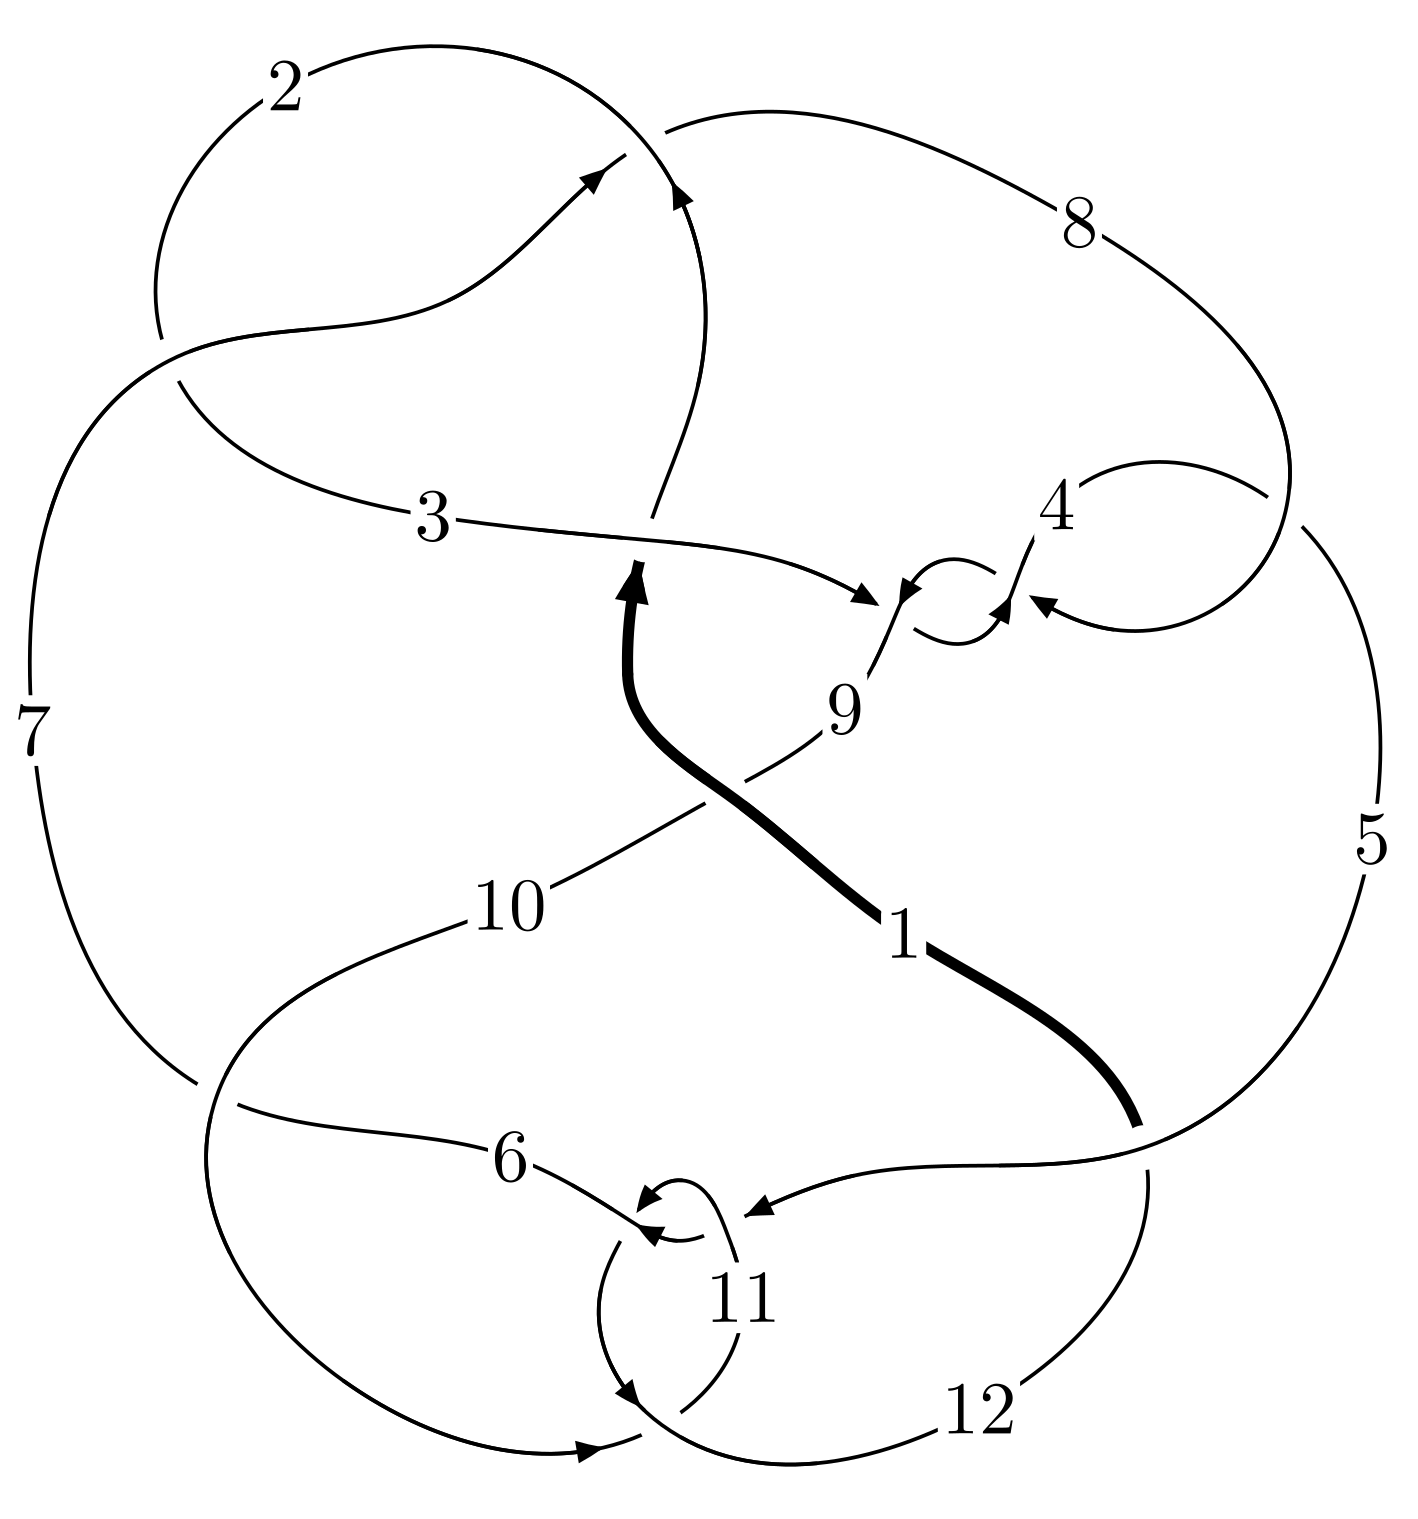
\includegraphics[width=112pt]{../../../GIT/diagram.site/Diagrams/png/1363_12a_0562.png}\\
\ \ \ A knot diagram\footnotemark}&
\allowdisplaybreaks
\textbf{Linearized knot diagam} \\
\cline{2-2}
 &
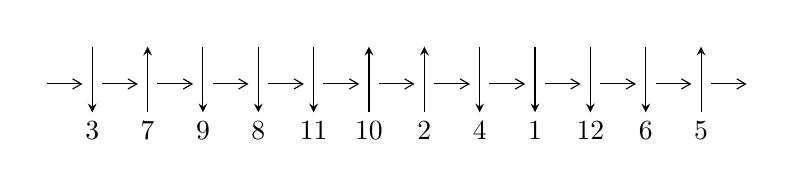
\begin{tikzpicture}[x=20pt, y=17pt]
	% nodes
	\node (C0) at (0, 0) {};
	\node (C1) at (1, 0) {};
	\node (C1U) at (1, +1) {};
	\node (C1D) at (1, -1) {3};

	\node (C2) at (2, 0) {};
	\node (C2U) at (2, +1) {};
	\node (C2D) at (2, -1) {7};

	\node (C3) at (3, 0) {};
	\node (C3U) at (3, +1) {};
	\node (C3D) at (3, -1) {9};

	\node (C4) at (4, 0) {};
	\node (C4U) at (4, +1) {};
	\node (C4D) at (4, -1) {8};

	\node (C5) at (5, 0) {};
	\node (C5U) at (5, +1) {};
	\node (C5D) at (5, -1) {11};

	\node (C6) at (6, 0) {};
	\node (C6U) at (6, +1) {};
	\node (C6D) at (6, -1) {10};

	\node (C7) at (7, 0) {};
	\node (C7U) at (7, +1) {};
	\node (C7D) at (7, -1) {2};

	\node (C8) at (8, 0) {};
	\node (C8U) at (8, +1) {};
	\node (C8D) at (8, -1) {4};

	\node (C9) at (9, 0) {};
	\node (C9U) at (9, +1) {};
	\node (C9D) at (9, -1) {1};

	\node (C10) at (10, 0) {};
	\node (C10U) at (10, +1) {};
	\node (C10D) at (10, -1) {12};

	\node (C11) at (11, 0) {};
	\node (C11U) at (11, +1) {};
	\node (C11D) at (11, -1) {6};

	\node (C12) at (12, 0) {};
	\node (C12U) at (12, +1) {};
	\node (C12D) at (12, -1) {5};
	\node (C13) at (13, 0) {};

	% arrows
	\draw[->,>={angle 60}]
	(C0) edge (C1) (C1) edge (C2) (C2) edge (C3) (C3) edge (C4) (C4) edge (C5) (C5) edge (C6) (C6) edge (C7) (C7) edge (C8) (C8) edge (C9) (C9) edge (C10) (C10) edge (C11) (C11) edge (C12) (C12) edge (C13) ;	\draw[->,>=stealth]
	(C1U) edge (C1D) (C2D) edge (C2U) (C3U) edge (C3D) (C4U) edge (C4D) (C5U) edge (C5D) (C6D) edge (C6U) (C7D) edge (C7U) (C8U) edge (C8D) (C9U) edge (C9D) (C10U) edge (C10D) (C11U) edge (C11D) (C12D) edge (C12U) ;
	\end{tikzpicture} \\
\hhline{~~} \\& 
\textbf{Solving Sequence} \\ \cline{2-2} 
 &
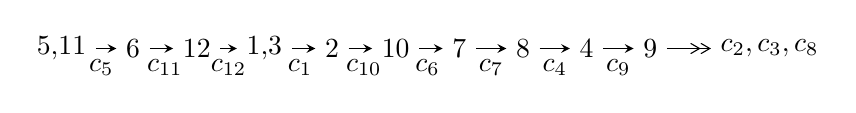
\begin{tikzpicture}[x=23pt, y=7pt]
	% node
	\node (A0) at (-1/8, 0) {5,11};
	\node (A1) at (1, 0) {6};
	\node (A2) at (2, 0) {12};
	\node (A3) at (49/16, 0) {1,3};
	\node (A4) at (33/8, 0) {2};
	\node (A5) at (41/8, 0) {10};
	\node (A6) at (49/8, 0) {7};
	\node (A7) at (57/8, 0) {8};
	\node (A8) at (65/8, 0) {4};
	\node (A9) at (73/8, 0) {9};
	\node (C1) at (1/2, -1) {$c_{5}$};
	\node (C2) at (3/2, -1) {$c_{11}$};
	\node (C3) at (5/2, -1) {$c_{12}$};
	\node (C4) at (29/8, -1) {$c_{1}$};
	\node (C5) at (37/8, -1) {$c_{10}$};
	\node (C6) at (45/8, -1) {$c_{6}$};
	\node (C7) at (53/8, -1) {$c_{7}$};
	\node (C8) at (61/8, -1) {$c_{4}$};
	\node (C9) at (69/8, -1) {$c_{9}$};
	\node (A10) at (11, 0) {$c_{2},c_{3},c_{8}$};

	% edge
	\draw[->,>=stealth]	
	(A0) edge (A1) (A1) edge (A2) (A2) edge (A3) (A3) edge (A4) (A4) edge (A5) (A5) edge (A6) (A6) edge (A7) (A7) edge (A8) (A8) edge (A9) ;
	\draw[->>,>={angle 60}]	
	(A9) edge (A10);
\end{tikzpicture} \\ 

\end{tabular} \\

\footnotetext{
The image of knot diagram is generated by the software ``\textbf{Draw programme}" developed by Andrew Bartholomew(\url{http://www.layer8.co.uk/maths/draw/index.htm\#Running-draw}), where we modified some parts for our purpose(\url{https://github.com/CATsTAILs/LinksPainter}).
}\phantom \\ \newline 
\centering \textbf{Ideals for irreducible components\footnotemark of $X_{\text{par}}$} 
 
\begin{align*}
I^u_{1}&=\langle 
3 u^{60}-48 u^{58}+\cdots+4 b+4,\;2 u^{67}-36 u^{65}+\cdots+4 a-4,\;u^{68}+2 u^{67}+\cdots+5 u+2\rangle \\
I^u_{2}&=\langle 
-2319 u^8 a^2-1264 u^8 a+\cdots+708 a+1030,\;5 u^8 a+u^8+\cdots-3 a-3,\\
\phantom{I^u_{2}}&\phantom{= \langle  }u^9- u^8-2 u^7+3 u^6+u^5-3 u^4+2 u^3- u+1\rangle \\
I^u_{3}&=\langle 
b-1,\;u^8+u^7-2 u^6-2 u^5+2 u^4+2 u^3+u^2+a+u-1,\;u^{10}-3 u^8+4 u^6- u^4- u^2+1\rangle \\
\\
\end{align*}
\raggedright * 3 irreducible components of $\dim_{\mathbb{C}}=0$, with total 105 representations.\\
\footnotetext{All coefficients of polynomials are rational numbers. But the coefficients are sometimes approximated in decimal forms when there is not enough margin.}
\newpage
\renewcommand{\arraystretch}{1}
\centering \section*{I. $I^u_{1}= \langle 3 u^{60}-48 u^{58}+\cdots+4 b+4,\;2 u^{67}-36 u^{65}+\cdots+4 a-4,\;u^{68}+2 u^{67}+\cdots+5 u+2 \rangle$}
\flushleft \textbf{(i) Arc colorings}\\
\begin{tabular}{m{7pt} m{180pt} m{7pt} m{180pt} }
\flushright $a_{5}=$&$\begin{pmatrix}1\\0\end{pmatrix}$ \\
\flushright $a_{11}=$&$\begin{pmatrix}0\\u\end{pmatrix}$ \\
\flushright $a_{6}=$&$\begin{pmatrix}1\\u^2\end{pmatrix}$ \\
\flushright $a_{12}=$&$\begin{pmatrix}- u\\- u^3+u\end{pmatrix}$ \\
\flushright $a_{1}=$&$\begin{pmatrix}- u^3\\- u^3+u\end{pmatrix}$ \\
\flushright $a_{3}=$&$\begin{pmatrix}-\frac{1}{2} u^{67}+9 u^{65}+\cdots-\frac{1}{4} u+1\\-\frac{3}{4} u^{60}+12 u^{58}+\cdots+\frac{1}{2} u-1\end{pmatrix}$ \\
\flushright $a_{2}=$&$\begin{pmatrix}-\frac{1}{4} u^{60}+\frac{15}{4} u^{58}+\cdots-\frac{1}{2} u+\frac{1}{2}\\-\frac{1}{4} u^{60}+4 u^{58}+\cdots-\frac{5}{4} u^2+u\end{pmatrix}$ \\
\flushright $a_{10}=$&$\begin{pmatrix}u^3\\u^5- u^3+u\end{pmatrix}$ \\
\flushright $a_{7}=$&$\begin{pmatrix}u^6- u^4+1\\u^8-2 u^6+2 u^4\end{pmatrix}$ \\
\flushright $a_{8}=$&$\begin{pmatrix}-\frac{1}{2} u^{67}-\frac{1}{4} u^{66}+\cdots-\frac{11}{4} u^2-\frac{7}{4} u\\-\frac{1}{2} u^{67}-\frac{1}{2} u^{66}+\cdots-\frac{9}{4} u-\frac{1}{2}\end{pmatrix}$ \\
\flushright $a_{4}=$&$\begin{pmatrix}\frac{1}{4} u^{55}-\frac{7}{2} u^{53}+\cdots+\frac{3}{4} u+1\\\frac{1}{4} u^{57}-\frac{15}{4} u^{55}+\cdots-\frac{1}{2} u^2+\frac{1}{2} u\end{pmatrix}$ \\
\flushright $a_{9}=$&$\begin{pmatrix}u^{11}-2 u^9+2 u^7+u^3\\u^{11}-3 u^9+4 u^7- u^5- u^3+u\end{pmatrix}$\\&\end{tabular}
\flushleft \textbf{(ii) Obstruction class $= -1$}\\~\\
\flushleft \textbf{(iii) Cusp Shapes $= -2 u^{67}+36 u^{65}+\cdots-12 u-2$}\\~\\
\newpage\renewcommand{\arraystretch}{1}
\flushleft \textbf{(iv) u-Polynomials at the component}\newline \\
\begin{tabular}{m{50pt}|m{274pt}}
Crossings & \hspace{64pt}u-Polynomials at each crossing \\
\hline $$\begin{aligned}c_{1}\end{aligned}$$&$\begin{aligned}
&u^{68}+27 u^{67}+\cdots+7896 u+289
\end{aligned}$\\
\hline $$\begin{aligned}c_{2},c_{7}\end{aligned}$$&$\begin{aligned}
&u^{68}+u^{67}+\cdots-20 u+17
\end{aligned}$\\
\hline $$\begin{aligned}c_{3},c_{4},c_{8}\end{aligned}$$&$\begin{aligned}
&u^{68}+u^{67}+\cdots-42 u+17
\end{aligned}$\\
\hline $$\begin{aligned}c_{5},c_{11}\end{aligned}$$&$\begin{aligned}
&u^{68}+2 u^{67}+\cdots+5 u+2
\end{aligned}$\\
\hline $$\begin{aligned}c_{6},c_{12}\end{aligned}$$&$\begin{aligned}
&u^{68}+6 u^{67}+\cdots+160 u+128
\end{aligned}$\\
\hline $$\begin{aligned}c_{9}\end{aligned}$$&$\begin{aligned}
&u^{68}-8 u^{67}+\cdots+28469 u+10016
\end{aligned}$\\
\hline $$\begin{aligned}c_{10}\end{aligned}$$&$\begin{aligned}
&u^{68}+36 u^{67}+\cdots-19 u+4
\end{aligned}$\\
\hline
\end{tabular}\\~\\
\newpage\renewcommand{\arraystretch}{1}
\flushleft \textbf{(v) Riley Polynomials at the component}\newline \\
\begin{tabular}{m{50pt}|m{274pt}}
Crossings & \hspace{64pt}Riley Polynomials at each crossing \\
\hline $$\begin{aligned}c_{1}\end{aligned}$$&$\begin{aligned}
&y^{68}+39 y^{67}+\cdots+6510324 y+83521
\end{aligned}$\\
\hline $$\begin{aligned}c_{2},c_{7}\end{aligned}$$&$\begin{aligned}
&y^{68}+27 y^{67}+\cdots+7896 y+289
\end{aligned}$\\
\hline $$\begin{aligned}c_{3},c_{4},c_{8}\end{aligned}$$&$\begin{aligned}
&y^{68}+71 y^{67}+\cdots-7272 y+289
\end{aligned}$\\
\hline $$\begin{aligned}c_{5},c_{11}\end{aligned}$$&$\begin{aligned}
&y^{68}-36 y^{67}+\cdots+19 y+4
\end{aligned}$\\
\hline $$\begin{aligned}c_{6},c_{12}\end{aligned}$$&$\begin{aligned}
&y^{68}+52 y^{67}+\cdots+1088512 y+16384
\end{aligned}$\\
\hline $$\begin{aligned}c_{9}\end{aligned}$$&$\begin{aligned}
&y^{68}+8 y^{67}+\cdots+482721863 y+100320256
\end{aligned}$\\
\hline $$\begin{aligned}c_{10}\end{aligned}$$&$\begin{aligned}
&y^{68}-8 y^{67}+\cdots-417 y+16
\end{aligned}$\\
\hline
\end{tabular}\\~\\
\newpage\flushleft \textbf{(vi) Complex Volumes and Cusp Shapes}
$$\begin{array}{c|c|c}  
\text{Solutions to }I^u_{1}& \I (\text{vol} + \sqrt{-1}CS) & \text{Cusp shape}\\
 \hline 
\begin{aligned}
u &= -0.840906 + 0.541453 I \\
a &= -1.68268 - 0.94647 I \\
b &= -0.79895 + 1.76961 I\end{aligned}
 & \phantom{-}0.64575 + 6.76137 I & -3.02362 - 9.36135 I \\ \hline\begin{aligned}
u &= -0.840906 - 0.541453 I \\
a &= -1.68268 + 0.94647 I \\
b &= -0.79895 - 1.76961 I\end{aligned}
 & \phantom{-}0.64575 - 6.76137 I & -3.02362 + 9.36135 I \\ \hline\begin{aligned}
u &= \phantom{-}0.996210 + 0.105534 I \\
a &= -0.88720 - 1.68128 I \\
b &= -0.755001 - 0.743583 I\end{aligned}
 & -3.62273 - 3.17922 I & -12.49077 + 5.37603 I \\ \hline\begin{aligned}
u &= \phantom{-}0.996210 - 0.105534 I \\
a &= -0.88720 + 1.68128 I \\
b &= -0.755001 + 0.743583 I\end{aligned}
 & -3.62273 + 3.17922 I & -12.49077 - 5.37603 I \\ \hline\begin{aligned}
u &= -0.827181 + 0.584200 I \\
a &= \phantom{-}0.631027 + 0.169558 I \\
b &= -0.131814 - 1.265700 I\end{aligned}
 & \phantom{-}8.49998 + 4.71847 I & \phantom{-}2.64745 - 4.37235 I \\ \hline\begin{aligned}
u &= -0.827181 - 0.584200 I \\
a &= \phantom{-}0.631027 - 0.169558 I \\
b &= -0.131814 + 1.265700 I\end{aligned}
 & \phantom{-}8.49998 - 4.71847 I & \phantom{-}2.64745 + 4.37235 I \\ \hline\begin{aligned}
u &= \phantom{-}0.865742 + 0.583006 I \\
a &= \phantom{-}1.67800 - 0.77268 I \\
b &= \phantom{-}0.55259 + 1.85985 I\end{aligned}
 & \phantom{-}6.64125 - 10.66220 I & \phantom{-0.000000 -}0. + 8.92755 I \\ \hline\begin{aligned}
u &= \phantom{-}0.865742 - 0.583006 I \\
a &= \phantom{-}1.67800 + 0.77268 I \\
b &= \phantom{-}0.55259 - 1.85985 I\end{aligned}
 & \phantom{-}6.64125 + 10.66220 I & \phantom{-0.000000 } 0. - 8.92755 I \\ \hline\begin{aligned}
u &= -0.884770 + 0.361343 I \\
a &= \phantom{-}1.31924 - 0.62047 I \\
b &= -0.0505122 - 0.1233410 I\end{aligned}
 & -2.02149 + 1.35661 I & -10.70049 - 3.21023 I \\ \hline\begin{aligned}
u &= -0.884770 - 0.361343 I \\
a &= \phantom{-}1.31924 + 0.62047 I \\
b &= -0.0505122 + 0.1233410 I\end{aligned}
 & -2.02149 - 1.35661 I & -10.70049 + 3.21023 I\\
 \hline 
 \end{array}$$\newpage$$\begin{array}{c|c|c}  
\text{Solutions to }I^u_{1}& \I (\text{vol} + \sqrt{-1}CS) & \text{Cusp shape}\\
 \hline 
\begin{aligned}
u &= -0.704686 + 0.598885 I \\
a &= -1.231360 - 0.615484 I \\
b &= -0.287687 + 1.027190 I\end{aligned}
 & \phantom{-}8.85003 - 0.06365 I & \phantom{-}3.56810 - 2.34699 I \\ \hline\begin{aligned}
u &= -0.704686 - 0.598885 I \\
a &= -1.231360 + 0.615484 I \\
b &= -0.287687 - 1.027190 I\end{aligned}
 & \phantom{-}8.85003 + 0.06365 I & \phantom{-}3.56810 + 2.34699 I \\ \hline\begin{aligned}
u &= \phantom{-}0.654533 + 0.611050 I \\
a &= -1.293350 + 0.557244 I \\
b &= \phantom{-}0.37269 - 1.71190 I\end{aligned}
 & \phantom{-}7.24282 + 5.98050 I & \phantom{-}1.58701 - 2.73296 I \\ \hline\begin{aligned}
u &= \phantom{-}0.654533 - 0.611050 I \\
a &= -1.293350 - 0.557244 I \\
b &= \phantom{-}0.37269 + 1.71190 I\end{aligned}
 & \phantom{-}7.24282 - 5.98050 I & \phantom{-}1.58701 + 2.73296 I \\ \hline\begin{aligned}
u &= -1.097730 + 0.129973 I \\
a &= \phantom{-}0.66528 - 1.74507 I \\
b &= \phantom{-}0.610710 - 1.198750 I\end{aligned}
 & \phantom{-}1.58150 + 6.31789 I & \phantom{-0.000000 } 0 \\ \hline\begin{aligned}
u &= -1.097730 - 0.129973 I \\
a &= \phantom{-}0.66528 + 1.74507 I \\
b &= \phantom{-}0.610710 + 1.198750 I\end{aligned}
 & \phantom{-}1.58150 - 6.31789 I & \phantom{-0.000000 } 0 \\ \hline\begin{aligned}
u &= \phantom{-}1.088810 + 0.220966 I \\
a &= -0.577505 + 0.470525 I \\
b &= \phantom{-}0.156355 + 0.374983 I\end{aligned}
 & \phantom{-}2.95364 - 1.17645 I & \phantom{-0.000000 } 0 \\ \hline\begin{aligned}
u &= \phantom{-}1.088810 - 0.220966 I \\
a &= -0.577505 - 0.470525 I \\
b &= \phantom{-}0.156355 - 0.374983 I\end{aligned}
 & \phantom{-}2.95364 + 1.17645 I & \phantom{-0.000000 } 0 \\ \hline\begin{aligned}
u &= -0.675962 + 0.538934 I \\
a &= \phantom{-}1.46405 + 0.27481 I \\
b &= -0.45008 - 1.66037 I\end{aligned}
 & \phantom{-}1.11309 - 2.39299 I & -1.31545 + 2.74693 I \\ \hline\begin{aligned}
u &= -0.675962 - 0.538934 I \\
a &= \phantom{-}1.46405 - 0.27481 I \\
b &= -0.45008 + 1.66037 I\end{aligned}
 & \phantom{-}1.11309 + 2.39299 I & -1.31545 - 2.74693 I\\
 \hline 
 \end{array}$$\newpage$$\begin{array}{c|c|c}  
\text{Solutions to }I^u_{1}& \I (\text{vol} + \sqrt{-1}CS) & \text{Cusp shape}\\
 \hline 
\begin{aligned}
u &= \phantom{-}0.753612 + 0.388922 I \\
a &= -0.003675 - 0.950130 I \\
b &= \phantom{-}0.929815 - 0.107409 I\end{aligned}
 & \phantom{-}1.24035 - 1.74892 I & \phantom{-}3.03511 + 5.28030 I \\ \hline\begin{aligned}
u &= \phantom{-}0.753612 - 0.388922 I \\
a &= -0.003675 + 0.950130 I \\
b &= \phantom{-}0.929815 + 0.107409 I\end{aligned}
 & \phantom{-}1.24035 + 1.74892 I & \phantom{-}3.03511 - 5.28030 I \\ \hline\begin{aligned}
u &= \phantom{-}0.165754 + 0.823138 I \\
a &= \phantom{-}1.002930 + 0.124969 I \\
b &= \phantom{-}0.98242 - 1.90847 I\end{aligned}
 & \phantom{-}3.07394 + 11.57570 I & -1.74839 - 6.82824 I \\ \hline\begin{aligned}
u &= \phantom{-}0.165754 - 0.823138 I \\
a &= \phantom{-}1.002930 - 0.124969 I \\
b &= \phantom{-}0.98242 + 1.90847 I\end{aligned}
 & \phantom{-}3.07394 - 11.57570 I & -1.74839 + 6.82824 I \\ \hline\begin{aligned}
u &= \phantom{-}0.029718 + 0.835469 I \\
a &= -0.311656 + 0.504146 I \\
b &= \phantom{-}0.691747 + 0.421141 I\end{aligned}
 & -1.00288 - 1.92318 I & -1.79190 + 3.81342 I \\ \hline\begin{aligned}
u &= \phantom{-}0.029718 - 0.835469 I \\
a &= -0.311656 - 0.504146 I \\
b &= \phantom{-}0.691747 - 0.421141 I\end{aligned}
 & -1.00288 + 1.92318 I & -1.79190 - 3.81342 I \\ \hline\begin{aligned}
u &= -0.183684 + 0.797547 I \\
a &= \phantom{-}0.279594 - 0.071647 I \\
b &= \phantom{-}0.35544 + 1.52101 I\end{aligned}
 & \phantom{-}5.39105 - 5.75675 I & \phantom{-}1.12004 + 2.96362 I \\ \hline\begin{aligned}
u &= -0.183684 - 0.797547 I \\
a &= \phantom{-}0.279594 + 0.071647 I \\
b &= \phantom{-}0.35544 - 1.52101 I\end{aligned}
 & \phantom{-}5.39105 + 5.75675 I & \phantom{-}1.12004 - 2.96362 I \\ \hline\begin{aligned}
u &= \phantom{-}1.072680 + 0.514608 I \\
a &= -2.06130 - 0.56028 I \\
b &= -0.090665 - 1.048220 I\end{aligned}
 & \phantom{-}3.97397 - 0.25739 I & \phantom{-0.000000 } 0 \\ \hline\begin{aligned}
u &= \phantom{-}1.072680 - 0.514608 I \\
a &= -2.06130 + 0.56028 I \\
b &= -0.090665 + 1.048220 I\end{aligned}
 & \phantom{-}3.97397 + 0.25739 I & \phantom{-0.000000 } 0\\
 \hline 
 \end{array}$$\newpage$$\begin{array}{c|c|c}  
\text{Solutions to }I^u_{1}& \I (\text{vol} + \sqrt{-1}CS) & \text{Cusp shape}\\
 \hline 
\begin{aligned}
u &= -0.151153 + 0.793214 I \\
a &= -1.085160 + 0.133068 I \\
b &= -1.39874 - 1.64237 I\end{aligned}
 & -2.51385 - 7.29843 I & -5.32805 + 6.53927 I \\ \hline\begin{aligned}
u &= -0.151153 - 0.793214 I \\
a &= -1.085160 - 0.133068 I \\
b &= -1.39874 + 1.64237 I\end{aligned}
 & -2.51385 + 7.29843 I & -5.32805 - 6.53927 I \\ \hline\begin{aligned}
u &= -0.061331 + 0.780735 I \\
a &= \phantom{-}0.330547 + 0.805383 I \\
b &= -0.502018 - 0.085930 I\end{aligned}
 & -4.88006 - 0.19763 I & -10.23533 - 0.14539 I \\ \hline\begin{aligned}
u &= -0.061331 - 0.780735 I \\
a &= \phantom{-}0.330547 - 0.805383 I \\
b &= -0.502018 + 0.085930 I\end{aligned}
 & -4.88006 + 0.19763 I & -10.23533 + 0.14539 I \\ \hline\begin{aligned}
u &= \phantom{-}1.147840 + 0.446072 I \\
a &= \phantom{-}0.78870 - 2.15745 I \\
b &= \phantom{-}1.10678 - 0.89125 I\end{aligned}
 & -3.04492 - 5.41261 I & \phantom{-0.000000 } 0 \\ \hline\begin{aligned}
u &= \phantom{-}1.147840 - 0.446072 I \\
a &= \phantom{-}0.78870 + 2.15745 I \\
b &= \phantom{-}1.10678 + 0.89125 I\end{aligned}
 & -3.04492 + 5.41261 I & \phantom{-0.000000 } 0 \\ \hline\begin{aligned}
u &= -1.116720 + 0.521286 I \\
a &= -1.57151 - 0.51789 I \\
b &= -0.573997 + 0.218690 I\end{aligned}
 & \phantom{-}4.70746 + 6.09415 I & \phantom{-0.000000 } 0 \\ \hline\begin{aligned}
u &= -1.116720 - 0.521286 I \\
a &= -1.57151 + 0.51789 I \\
b &= -0.573997 - 0.218690 I\end{aligned}
 & \phantom{-}4.70746 - 6.09415 I & \phantom{-0.000000 } 0 \\ \hline\begin{aligned}
u &= -1.142120 + 0.472829 I \\
a &= \phantom{-}2.64269 - 0.71234 I \\
b &= \phantom{-}0.73682 - 1.37957 I\end{aligned}
 & -2.86459 + 2.56142 I & \phantom{-0.000000 } 0 \\ \hline\begin{aligned}
u &= -1.142120 - 0.472829 I \\
a &= \phantom{-}2.64269 + 0.71234 I \\
b &= \phantom{-}0.73682 + 1.37957 I\end{aligned}
 & -2.86459 - 2.56142 I & \phantom{-0.000000 } 0\\
 \hline 
 \end{array}$$\newpage$$\begin{array}{c|c|c}  
\text{Solutions to }I^u_{1}& \I (\text{vol} + \sqrt{-1}CS) & \text{Cusp shape}\\
 \hline 
\begin{aligned}
u &= -0.288870 + 0.702347 I \\
a &= -0.974335 + 0.183643 I \\
b &= -0.386475 - 0.456700 I\end{aligned}
 & \phantom{-}7.11141 - 1.43004 I & \phantom{-}2.66134 + 2.04753 I \\ \hline\begin{aligned}
u &= -0.288870 - 0.702347 I \\
a &= -0.974335 - 0.183643 I \\
b &= -0.386475 + 0.456700 I\end{aligned}
 & \phantom{-}7.11141 + 1.43004 I & \phantom{-}2.66134 - 2.04753 I \\ \hline\begin{aligned}
u &= \phantom{-}0.357888 + 0.667374 I \\
a &= -0.889683 - 0.281502 I \\
b &= \phantom{-}0.141604 + 1.285040 I\end{aligned}
 & \phantom{-}6.03868 - 4.30670 I & \phantom{-}1.46994 + 3.45796 I \\ \hline\begin{aligned}
u &= \phantom{-}0.357888 - 0.667374 I \\
a &= -0.889683 + 0.281502 I \\
b &= \phantom{-}0.141604 - 1.285040 I\end{aligned}
 & \phantom{-}6.03868 + 4.30670 I & \phantom{-}1.46994 - 3.45796 I \\ \hline\begin{aligned}
u &= \phantom{-}1.197530 + 0.346738 I \\
a &= -0.11563 - 1.85593 I \\
b &= \phantom{-}0.55742 - 1.36973 I\end{aligned}
 & \phantom{-}1.21003 + 2.01792 I & \phantom{-0.000000 } 0 \\ \hline\begin{aligned}
u &= \phantom{-}1.197530 - 0.346738 I \\
a &= -0.11563 + 1.85593 I \\
b &= \phantom{-}0.55742 + 1.36973 I\end{aligned}
 & \phantom{-}1.21003 - 2.01792 I & \phantom{-0.000000 } 0 \\ \hline\begin{aligned}
u &= \phantom{-}1.202190 + 0.372091 I \\
a &= -1.56784 + 2.63243 I \\
b &= -1.49112 + 1.42833 I\end{aligned}
 & -6.55660 + 3.40545 I & \phantom{-0.000000 } 0 \\ \hline\begin{aligned}
u &= \phantom{-}1.202190 - 0.372091 I \\
a &= -1.56784 - 2.63243 I \\
b &= -1.49112 - 1.42833 I\end{aligned}
 & -6.55660 - 3.40545 I & \phantom{-0.000000 } 0 \\ \hline\begin{aligned}
u &= -1.221200 + 0.356970 I \\
a &= \phantom{-}0.89428 + 2.61237 I \\
b &= \phantom{-}1.06051 + 1.77150 I\end{aligned}
 & -1.16641 - 7.64309 I & \phantom{-0.000000 } 0 \\ \hline\begin{aligned}
u &= -1.221200 - 0.356970 I \\
a &= \phantom{-}0.89428 - 2.61237 I \\
b &= \phantom{-}1.06051 - 1.77150 I\end{aligned}
 & -1.16641 + 7.64309 I & \phantom{-0.000000 } 0\\
 \hline 
 \end{array}$$\newpage$$\begin{array}{c|c|c}  
\text{Solutions to }I^u_{1}& \I (\text{vol} + \sqrt{-1}CS) & \text{Cusp shape}\\
 \hline 
\begin{aligned}
u &= \phantom{-}1.204100 + 0.423605 I \\
a &= -0.348738 - 0.171647 I \\
b &= -0.652313 + 0.123062 I\end{aligned}
 & -8.58591 - 4.02293 I & \phantom{-0.000000 } 0 \\ \hline\begin{aligned}
u &= \phantom{-}1.204100 - 0.423605 I \\
a &= -0.348738 + 0.171647 I \\
b &= -0.652313 - 0.123062 I\end{aligned}
 & -8.58591 + 4.02293 I & \phantom{-0.000000 } 0 \\ \hline\begin{aligned}
u &= -1.197470 + 0.478507 I \\
a &= -0.235493 - 0.884755 I \\
b &= -0.457387 + 0.202512 I\end{aligned}
 & -8.19611 + 4.78252 I & \phantom{-0.000000 } 0 \\ \hline\begin{aligned}
u &= -1.197470 - 0.478507 I \\
a &= -0.235493 + 0.884755 I \\
b &= -0.457387 - 0.202512 I\end{aligned}
 & -8.19611 - 4.78252 I & \phantom{-0.000000 } 0 \\ \hline\begin{aligned}
u &= -1.180790 + 0.525663 I \\
a &= \phantom{-}2.06732 - 0.85708 I \\
b &= \phantom{-}0.42377 - 1.66754 I\end{aligned}
 & \phantom{-}2.45212 + 10.65030 I & \phantom{-0.000000 } 0 \\ \hline\begin{aligned}
u &= -1.180790 - 0.525663 I \\
a &= \phantom{-}2.06732 + 0.85708 I \\
b &= \phantom{-}0.42377 + 1.66754 I\end{aligned}
 & \phantom{-}2.45212 - 10.65030 I & \phantom{-0.000000 } 0 \\ \hline\begin{aligned}
u &= -1.187140 + 0.513961 I \\
a &= -3.70852 - 0.08255 I \\
b &= -1.53628 + 1.72826 I\end{aligned}
 & -5.55900 + 12.12010 I & \phantom{-0.000000 } 0 \\ \hline\begin{aligned}
u &= -1.187140 - 0.513961 I \\
a &= -3.70852 + 0.08255 I \\
b &= -1.53628 - 1.72826 I\end{aligned}
 & -5.55900 - 12.12010 I & \phantom{-0.000000 } 0 \\ \hline\begin{aligned}
u &= \phantom{-}1.194400 + 0.526145 I \\
a &= \phantom{-}3.44519 + 0.50306 I \\
b &= \phantom{-}1.06198 + 1.98167 I\end{aligned}
 & \phantom{-}0.0245 - 16.5311 I & \phantom{-0.000000 } 0 \\ \hline\begin{aligned}
u &= \phantom{-}1.194400 - 0.526145 I \\
a &= \phantom{-}3.44519 - 0.50306 I \\
b &= \phantom{-}1.06198 - 1.98167 I\end{aligned}
 & \phantom{-}0.0245 + 16.5311 I & \phantom{-0.000000 } 0\\
 \hline 
 \end{array}$$\newpage$$\begin{array}{c|c|c}  
\text{Solutions to }I^u_{1}& \I (\text{vol} + \sqrt{-1}CS) & \text{Cusp shape}\\
 \hline 
\begin{aligned}
u &= -1.231000 + 0.440784 I \\
a &= \phantom{-}0.823478 - 0.382539 I \\
b &= \phantom{-}0.770134 - 0.469099 I\end{aligned}
 & -4.78562 + 6.43179 I & \phantom{-0.000000 } 0 \\ \hline\begin{aligned}
u &= -1.231000 - 0.440784 I \\
a &= \phantom{-}0.823478 + 0.382539 I \\
b &= \phantom{-}0.770134 + 0.469099 I\end{aligned}
 & -4.78562 - 6.43179 I & \phantom{-0.000000 } 0 \\ \hline\begin{aligned}
u &= \phantom{-}1.224950 + 0.470945 I \\
a &= \phantom{-}0.064399 - 1.290010 I \\
b &= \phantom{-}0.726960 - 0.347094 I\end{aligned}
 & -4.57008 - 2.76226 I & \phantom{-0.000000 } 0 \\ \hline\begin{aligned}
u &= \phantom{-}1.224950 - 0.470945 I \\
a &= \phantom{-}0.064399 + 1.290010 I \\
b &= \phantom{-}0.726960 + 0.347094 I\end{aligned}
 & -4.57008 + 2.76226 I & \phantom{-0.000000 } 0 \\ \hline\begin{aligned}
u &= -0.225662 + 0.547625 I \\
a &= \phantom{-}0.984096 + 0.221334 I \\
b &= \phantom{-}0.140194 + 1.076410 I\end{aligned}
 & -0.15904 + 1.57803 I & -1.93957 - 4.05866 I \\ \hline\begin{aligned}
u &= -0.225662 - 0.547625 I \\
a &= \phantom{-}0.984096 - 0.221334 I \\
b &= \phantom{-}0.140194 - 1.076410 I\end{aligned}
 & -0.15904 - 1.57803 I & -1.93957 + 4.05866 I \\ \hline\begin{aligned}
u &= \phantom{-}0.062422 + 0.547904 I \\
a &= \phantom{-}0.714824 + 0.515000 I \\
b &= \phantom{-}0.685106 + 0.637373 I\end{aligned}
 & -0.06279 + 1.44675 I & -0.83204 - 5.13904 I \\ \hline\begin{aligned}
u &= \phantom{-}0.062422 - 0.547904 I \\
a &= \phantom{-}0.714824 - 0.515000 I \\
b &= \phantom{-}0.685106 - 0.637373 I\end{aligned}
 & -0.06279 - 1.44675 I & -0.83204 + 5.13904 I\\
 \hline 
 \end{array}$$\newpage\newpage\renewcommand{\arraystretch}{1}
\centering \section*{II. $I^u_{2}= \langle -2319 u^8 a^2-1264 u^8 a+\cdots+708 a+1030,\;5 u^8 a+u^8+\cdots-3 a-3,\;u^9- u^8-2 u^7+3 u^6+u^5-3 u^4+2 u^3- u+1 \rangle$}
\flushleft \textbf{(i) Arc colorings}\\
\begin{tabular}{m{7pt} m{180pt} m{7pt} m{180pt} }
\flushright $a_{5}=$&$\begin{pmatrix}1\\0\end{pmatrix}$ \\
\flushright $a_{11}=$&$\begin{pmatrix}0\\u\end{pmatrix}$ \\
\flushright $a_{6}=$&$\begin{pmatrix}1\\u^2\end{pmatrix}$ \\
\flushright $a_{12}=$&$\begin{pmatrix}- u\\- u^3+u\end{pmatrix}$ \\
\flushright $a_{1}=$&$\begin{pmatrix}- u^3\\- u^3+u\end{pmatrix}$ \\
\flushright $a_{3}=$&$\begin{pmatrix}a\\1.00346 a^{2} u^{8}+0.546949 a u^{8}+\cdots-0.306361 a-0.445695\end{pmatrix}$ \\
\flushright $a_{2}=$&$\begin{pmatrix}0.0207702 a^{2} u^{8}-0.718304 a u^{8}+\cdots+1.16183 a+1.32583\\-0.0562527 a^{2} u^{8}+1.11207 a u^{8}+\cdots-0.0216357 a-1.25746\end{pmatrix}$ \\
\flushright $a_{10}=$&$\begin{pmatrix}u^3\\u^5- u^3+u\end{pmatrix}$ \\
\flushright $a_{7}=$&$\begin{pmatrix}u^6- u^4+1\\u^8-2 u^6+2 u^4\end{pmatrix}$ \\
\flushright $a_{8}=$&$\begin{pmatrix}1.60623 a^{2} u^{8}-0.215491 a u^{8}+\cdots-3.15145 a+1.19775\\-0.526179 a^{2} u^{8}-1.13630 a u^{8}+\cdots+0.566854 a+1.74556\end{pmatrix}$ \\
\flushright $a_{4}=$&$\begin{pmatrix}0.0207702 a^{2} u^{8}-0.718304 a u^{8}+\cdots+1.16183 a+1.32583\\-0.0562527 a^{2} u^{8}+1.11207 a u^{8}+\cdots-0.0216357 a-1.25746\end{pmatrix}$ \\
\flushright $a_{9}=$&$\begin{pmatrix}- u^6+u^4-1\\- u^8+2 u^6-2 u^4\end{pmatrix}$\\&\end{tabular}
\flushleft \textbf{(ii) Obstruction class $= -1$}\\~\\
\flushleft \textbf{(iii) Cusp Shapes $= 4 u^7-8 u^5+4 u^4+8 u^3-4 u^2+4 u-2$}\\~\\
\newpage\renewcommand{\arraystretch}{1}
\flushleft \textbf{(iv) u-Polynomials at the component}\newline \\
\begin{tabular}{m{50pt}|m{274pt}}
Crossings & \hspace{64pt}u-Polynomials at each crossing \\
\hline $$\begin{aligned}c_{1}\end{aligned}$$&$\begin{aligned}
&u^{27}+18 u^{26}+\cdots+u-1
\end{aligned}$\\
\hline $$\begin{aligned}c_{2},c_{3},c_{4}\\c_{7},c_{8}\end{aligned}$$&$\begin{aligned}
&u^{27}+9 u^{25}+\cdots+u+1
\end{aligned}$\\
\hline $$\begin{aligned}c_{5},c_{11}\end{aligned}$$&$\begin{aligned}
&(u^9- u^8-2 u^7+3 u^6+u^5-3 u^4+2 u^3- u+1)^3
\end{aligned}$\\
\hline $$\begin{aligned}c_{6},c_{12}\end{aligned}$$&$\begin{aligned}
&(u^9-3 u^8+8 u^7-13 u^6+17 u^5-17 u^4+12 u^3-6 u^2+u+1)^3
\end{aligned}$\\
\hline $$\begin{aligned}c_{9}\end{aligned}$$&$\begin{aligned}
&(u^9- u^8+2 u^7- u^6+3 u^5- u^4+2 u^3+u+1)^3
\end{aligned}$\\
\hline $$\begin{aligned}c_{10}\end{aligned}$$&$\begin{aligned}
&(u^9+5 u^8+12 u^7+15 u^6+9 u^5- u^4-4 u^3-2 u^2+u+1)^3
\end{aligned}$\\
\hline
\end{tabular}\\~\\
\newpage\renewcommand{\arraystretch}{1}
\flushleft \textbf{(v) Riley Polynomials at the component}\newline \\
\begin{tabular}{m{50pt}|m{274pt}}
Crossings & \hspace{64pt}Riley Polynomials at each crossing \\
\hline $$\begin{aligned}c_{1}\end{aligned}$$&$\begin{aligned}
&y^{27}-18 y^{26}+\cdots+17 y-1
\end{aligned}$\\
\hline $$\begin{aligned}c_{2},c_{3},c_{4}\\c_{7},c_{8}\end{aligned}$$&$\begin{aligned}
&y^{27}+18 y^{26}+\cdots+y-1
\end{aligned}$\\
\hline $$\begin{aligned}c_{5},c_{11}\end{aligned}$$&$\begin{aligned}
&(y^9-5 y^8+12 y^7-15 y^6+9 y^5+y^4-4 y^3+2 y^2+y-1)^3
\end{aligned}$\\
\hline $$\begin{aligned}c_{6},c_{12}\end{aligned}$$&$\begin{aligned}
&(y^9+7 y^8+20 y^7+25 y^6+5 y^5-15 y^4+22 y^2+13 y-1)^3
\end{aligned}$\\
\hline $$\begin{aligned}c_{9}\end{aligned}$$&$\begin{aligned}
&(y^9+3 y^8+8 y^7+13 y^6+17 y^5+17 y^4+12 y^3+6 y^2+y-1)^3
\end{aligned}$\\
\hline $$\begin{aligned}c_{10}\end{aligned}$$&$\begin{aligned}
&(y^9- y^8+12 y^7-7 y^6+37 y^5+y^4-10 y^2+5 y-1)^3
\end{aligned}$\\
\hline
\end{tabular}\\~\\
\newpage\flushleft \textbf{(vi) Complex Volumes and Cusp Shapes}
$$\begin{array}{c|c|c}  
\text{Solutions to }I^u_{2}& \I (\text{vol} + \sqrt{-1}CS) & \text{Cusp shape}\\
 \hline 
\begin{aligned}
u &= \phantom{-}0.772920 + 0.510351 I \\
a &= -1.015990 - 0.216914 I \\
b &= \phantom{-}0.53465 - 1.31702 I\end{aligned}
 & \phantom{-}1.78344 - 2.09337 I & \phantom{-}0.51499 + 4.16283 I \\ \hline\begin{aligned}
u &= \phantom{-}0.772920 + 0.510351 I \\
a &= -1.49846 - 0.72657 I \\
b &= \phantom{-}0.466265 + 0.129322 I\end{aligned}
 & \phantom{-}1.78344 - 2.09337 I & \phantom{-}0.51499 + 4.16283 I \\ \hline\begin{aligned}
u &= \phantom{-}0.772920 + 0.510351 I \\
a &= \phantom{-}1.25695 - 1.13794 I \\
b &= \phantom{-}0.99909 + 1.18770 I\end{aligned}
 & \phantom{-}1.78344 - 2.09337 I & \phantom{-}0.51499 + 4.16283 I \\ \hline\begin{aligned}
u &= \phantom{-}0.772920 - 0.510351 I \\
a &= -1.015990 + 0.216914 I \\
b &= \phantom{-}0.53465 + 1.31702 I\end{aligned}
 & \phantom{-}1.78344 + 2.09337 I & \phantom{-}0.51499 - 4.16283 I \\ \hline\begin{aligned}
u &= \phantom{-}0.772920 - 0.510351 I \\
a &= -1.49846 + 0.72657 I \\
b &= \phantom{-}0.466265 - 0.129322 I\end{aligned}
 & \phantom{-}1.78344 + 2.09337 I & \phantom{-}0.51499 - 4.16283 I \\ \hline\begin{aligned}
u &= \phantom{-}0.772920 - 0.510351 I \\
a &= \phantom{-}1.25695 + 1.13794 I \\
b &= \phantom{-}0.99909 - 1.18770 I\end{aligned}
 & \phantom{-}1.78344 + 2.09337 I & \phantom{-}0.51499 - 4.16283 I \\ \hline\begin{aligned}
u &= -0.825933\phantom{ +0.000000I} \\
a &= \phantom{-}0.164740\phantom{ +0.000000I} \\
b &= -0.407730\phantom{ +0.000000I}\end{aligned}
 & -1.19845\phantom{ +0.000000I} & -8.65230\phantom{ +0.000000I} \\ \hline\begin{aligned}
u &= -0.825933\phantom{ +0.000000I} \\
a &= \phantom{-}1.58072 + 1.94080 I \\
b &= \phantom{-}1.203870 - 0.085974 I\end{aligned}
 & -1.19845\phantom{ +0.000000I} & -8.65230\phantom{ +0.000000I} \\ \hline\begin{aligned}
u &= -0.825933\phantom{ +0.000000I} \\
a &= \phantom{-}1.58072 - 1.94080 I \\
b &= \phantom{-}1.203870 + 0.085974 I\end{aligned}
 & -1.19845\phantom{ +0.000000I} & -8.65230\phantom{ +0.000000I} \\ \hline\begin{aligned}
u &= -1.173910 + 0.391555 I \\
a &= \phantom{-}0.060301 + 0.267806 I \\
b &= \phantom{-}0.850678 + 0.663233 I\end{aligned}
 & -4.37135 + 1.33617 I & -7.28409 - 0.70175 I\\
 \hline 
 \end{array}$$\newpage$$\begin{array}{c|c|c}  
\text{Solutions to }I^u_{2}& \I (\text{vol} + \sqrt{-1}CS) & \text{Cusp shape}\\
 \hline 
\begin{aligned}
u &= -1.173910 + 0.391555 I \\
a &= -0.02187 - 1.90349 I \\
b &= -0.677531 - 1.190630 I\end{aligned}
 & -4.37135 + 1.33617 I & -7.28409 - 0.70175 I \\ \hline\begin{aligned}
u &= -1.173910 + 0.391555 I \\
a &= \phantom{-}2.60362 + 1.98656 I \\
b &= \phantom{-}1.82685 + 0.52740 I\end{aligned}
 & -4.37135 + 1.33617 I & -7.28409 - 0.70175 I \\ \hline\begin{aligned}
u &= -1.173910 - 0.391555 I \\
a &= \phantom{-}0.060301 - 0.267806 I \\
b &= \phantom{-}0.850678 - 0.663233 I\end{aligned}
 & -4.37135 - 1.33617 I & -7.28409 + 0.70175 I \\ \hline\begin{aligned}
u &= -1.173910 - 0.391555 I \\
a &= -0.02187 + 1.90349 I \\
b &= -0.677531 + 1.190630 I\end{aligned}
 & -4.37135 - 1.33617 I & -7.28409 + 0.70175 I \\ \hline\begin{aligned}
u &= -1.173910 - 0.391555 I \\
a &= \phantom{-}2.60362 - 1.98656 I \\
b &= \phantom{-}1.82685 - 0.52740 I\end{aligned}
 & -4.37135 - 1.33617 I & -7.28409 + 0.70175 I \\ \hline\begin{aligned}
u &= \phantom{-}0.141484 + 0.739668 I \\
a &= \phantom{-}1.137900 + 0.280832 I \\
b &= \phantom{-}1.68535 - 0.81163 I\end{aligned}
 & -0.61694 + 2.45442 I & -2.32792 - 2.91298 I \\ \hline\begin{aligned}
u &= \phantom{-}0.141484 + 0.739668 I \\
a &= -0.610565 + 1.028440 I \\
b &= \phantom{-}0.652744 - 0.562733 I\end{aligned}
 & -0.61694 + 2.45442 I & -2.32792 - 2.91298 I \\ \hline\begin{aligned}
u &= \phantom{-}0.141484 + 0.739668 I \\
a &= -0.363377 + 0.147221 I \\
b &= -0.33809 + 1.37436 I\end{aligned}
 & -0.61694 + 2.45442 I & -2.32792 - 2.91298 I \\ \hline\begin{aligned}
u &= \phantom{-}0.141484 - 0.739668 I \\
a &= \phantom{-}1.137900 - 0.280832 I \\
b &= \phantom{-}1.68535 + 0.81163 I\end{aligned}
 & -0.61694 - 2.45442 I & -2.32792 + 2.91298 I \\ \hline\begin{aligned}
u &= \phantom{-}0.141484 - 0.739668 I \\
a &= -0.610565 - 1.028440 I \\
b &= \phantom{-}0.652744 + 0.562733 I\end{aligned}
 & -0.61694 - 2.45442 I & -2.32792 + 2.91298 I\\
 \hline 
 \end{array}$$\newpage$$\begin{array}{c|c|c}  
\text{Solutions to }I^u_{2}& \I (\text{vol} + \sqrt{-1}CS) & \text{Cusp shape}\\
 \hline 
\begin{aligned}
u &= \phantom{-}0.141484 - 0.739668 I \\
a &= -0.363377 - 0.147221 I \\
b &= -0.33809 - 1.37436 I\end{aligned}
 & -0.61694 - 2.45442 I & -2.32792 + 2.91298 I \\ \hline\begin{aligned}
u &= \phantom{-}1.172470 + 0.500383 I \\
a &= \phantom{-}0.589040 - 0.774213 I \\
b &= \phantom{-}0.578755 + 0.699902 I\end{aligned}
 & -3.59813 - 7.08493 I & -5.57680 + 5.91335 I \\ \hline\begin{aligned}
u &= \phantom{-}1.172470 + 0.500383 I \\
a &= -2.17609 - 1.01614 I \\
b &= -0.46969 - 1.60732 I\end{aligned}
 & -3.59813 - 7.08493 I & -5.57680 + 5.91335 I \\ \hline\begin{aligned}
u &= \phantom{-}1.172470 + 0.500383 I \\
a &= \phantom{-}3.37545 - 1.16633 I \\
b &= \phantom{-}1.89094 + 0.90742 I\end{aligned}
 & -3.59813 - 7.08493 I & -5.57680 + 5.91335 I \\ \hline\begin{aligned}
u &= \phantom{-}1.172470 - 0.500383 I \\
a &= \phantom{-}0.589040 + 0.774213 I \\
b &= \phantom{-}0.578755 - 0.699902 I\end{aligned}
 & -3.59813 + 7.08493 I & -5.57680 - 5.91335 I \\ \hline\begin{aligned}
u &= \phantom{-}1.172470 - 0.500383 I \\
a &= -2.17609 + 1.01614 I \\
b &= -0.46969 + 1.60732 I\end{aligned}
 & -3.59813 + 7.08493 I & -5.57680 - 5.91335 I \\ \hline\begin{aligned}
u &= \phantom{-}1.172470 - 0.500383 I \\
a &= \phantom{-}3.37545 + 1.16633 I \\
b &= \phantom{-}1.89094 - 0.90742 I\end{aligned}
 & -3.59813 + 7.08493 I & -5.57680 - 5.91335 I\\
 \hline 
 \end{array}$$\newpage\newpage\renewcommand{\arraystretch}{1}
\centering \section*{III. $I^u_{3}= \langle b-1,\;u^8+u^7+\cdots+a-1,\;u^{10}-3 u^8+4 u^6- u^4- u^2+1 \rangle$}
\flushleft \textbf{(i) Arc colorings}\\
\begin{tabular}{m{7pt} m{180pt} m{7pt} m{180pt} }
\flushright $a_{5}=$&$\begin{pmatrix}1\\0\end{pmatrix}$ \\
\flushright $a_{11}=$&$\begin{pmatrix}0\\u\end{pmatrix}$ \\
\flushright $a_{6}=$&$\begin{pmatrix}1\\u^2\end{pmatrix}$ \\
\flushright $a_{12}=$&$\begin{pmatrix}- u\\- u^3+u\end{pmatrix}$ \\
\flushright $a_{1}=$&$\begin{pmatrix}- u^3\\- u^3+u\end{pmatrix}$ \\
\flushright $a_{3}=$&$\begin{pmatrix}- u^8- u^7+2 u^6+2 u^5-2 u^4-2 u^3- u^2- u+1\\1\end{pmatrix}$ \\
\flushright $a_{2}=$&$\begin{pmatrix}- u^8- u^7+2 u^6+2 u^5-2 u^4-3 u^3- u^2- u+1\\- u^3+u+1\end{pmatrix}$ \\
\flushright $a_{10}=$&$\begin{pmatrix}u^3\\u^5- u^3+u\end{pmatrix}$ \\
\flushright $a_{7}=$&$\begin{pmatrix}u^6- u^4+1\\u^8-2 u^6+2 u^4\end{pmatrix}$ \\
\flushright $a_{8}=$&$\begin{pmatrix}u^8- u^7-3 u^6+2 u^5+3 u^4- u^3+u^2- u-2\\- u^9+2 u^7- u^5-2 u^3+u\end{pmatrix}$ \\
\flushright $a_{4}=$&$\begin{pmatrix}- u^8- u^7+2 u^6+2 u^5-2 u^4-2 u^3- u^2- u+2\\1\end{pmatrix}$ \\
\flushright $a_{9}=$&$\begin{pmatrix}u^9-2 u^7+u^5+2 u^3- u\\0\end{pmatrix}$\\&\end{tabular}
\flushleft \textbf{(ii) Obstruction class $= 1$}\\~\\
\flushleft \textbf{(iii) Cusp Shapes $= 4 u^8-8 u^6+8 u^4+4 u^2-8$}\\~\\
\newpage\renewcommand{\arraystretch}{1}
\flushleft \textbf{(iv) u-Polynomials at the component}\newline \\
\begin{tabular}{m{50pt}|m{274pt}}
Crossings & \hspace{64pt}u-Polynomials at each crossing \\
\hline $$\begin{aligned}c_{1}\end{aligned}$$&$\begin{aligned}
&(u-1)^{10}
\end{aligned}$\\
\hline $$\begin{aligned}c_{2},c_{3},c_{4}\\c_{7},c_{8}\end{aligned}$$&$\begin{aligned}
&(u^2+1)^5
\end{aligned}$\\
\hline $$\begin{aligned}c_{5},c_{11}\end{aligned}$$&$\begin{aligned}
&u^{10}-3 u^8+4 u^6- u^4- u^2+1
\end{aligned}$\\
\hline $$\begin{aligned}c_{6},c_{12}\end{aligned}$$&$\begin{aligned}
&u^{10}+5 u^8+8 u^6+3 u^4- u^2+1
\end{aligned}$\\
\hline $$\begin{aligned}c_{9}\end{aligned}$$&$\begin{aligned}
&(u^5+u^4-2 u^3- u^2+u-1)^2
\end{aligned}$\\
\hline $$\begin{aligned}c_{10}\end{aligned}$$&$\begin{aligned}
&(u^5-3 u^4+4 u^3- u^2- u+1)^2
\end{aligned}$\\
\hline
\end{tabular}\\~\\
\newpage\renewcommand{\arraystretch}{1}
\flushleft \textbf{(v) Riley Polynomials at the component}\newline \\
\begin{tabular}{m{50pt}|m{274pt}}
Crossings & \hspace{64pt}Riley Polynomials at each crossing \\
\hline $$\begin{aligned}c_{1}\end{aligned}$$&$\begin{aligned}
&(y-1)^{10}
\end{aligned}$\\
\hline $$\begin{aligned}c_{2},c_{3},c_{4}\\c_{7},c_{8}\end{aligned}$$&$\begin{aligned}
&(y+1)^{10}
\end{aligned}$\\
\hline $$\begin{aligned}c_{5},c_{11}\end{aligned}$$&$\begin{aligned}
&(y^5-3 y^4+4 y^3- y^2- y+1)^2
\end{aligned}$\\
\hline $$\begin{aligned}c_{6},c_{12}\end{aligned}$$&$\begin{aligned}
&(y^5+5 y^4+8 y^3+3 y^2- y+1)^2
\end{aligned}$\\
\hline $$\begin{aligned}c_{9}\end{aligned}$$&$\begin{aligned}
&(y^5-5 y^4+8 y^3-3 y^2- y-1)^2
\end{aligned}$\\
\hline $$\begin{aligned}c_{10}\end{aligned}$$&$\begin{aligned}
&(y^5- y^4+8 y^3-3 y^2+3 y-1)^2
\end{aligned}$\\
\hline
\end{tabular}\\~\\
\newpage\flushleft \textbf{(vi) Complex Volumes and Cusp Shapes}
$$\begin{array}{c|c|c}  
\text{Solutions to }I^u_{3}& \I (\text{vol} + \sqrt{-1}CS) & \text{Cusp shape}\\
 \hline 
\begin{aligned}
u &= -0.822375 + 0.339110 I \\
a &= \phantom{-}1.50891 + 0.32986 I \\
b &= \phantom{-}1.00000\phantom{ +0.000000I}\end{aligned}
 & -0.32910 + 1.53058 I & -4.51511 - 4.43065 I \\ \hline\begin{aligned}
u &= -0.822375 - 0.339110 I \\
a &= \phantom{-}1.50891 - 0.32986 I \\
b &= \phantom{-}1.00000\phantom{ +0.000000I}\end{aligned}
 & -0.32910 - 1.53058 I & -4.51511 + 4.43065 I \\ \hline\begin{aligned}
u &= \phantom{-}0.822375 + 0.339110 I \\
a &= -1.25135 - 1.88547 I \\
b &= \phantom{-}1.00000\phantom{ +0.000000I}\end{aligned}
 & -0.32910 - 1.53058 I & -4.51511 + 4.43065 I \\ \hline\begin{aligned}
u &= \phantom{-}0.822375 - 0.339110 I \\
a &= -1.25135 + 1.88547 I \\
b &= \phantom{-}1.00000\phantom{ +0.000000I}\end{aligned}
 & -0.32910 + 1.53058 I & -4.51511 - 4.43065 I \\ \hline\begin{aligned}
u &= \phantom{-0.000000 -}0.766826 I \\
a &= \phantom{-}0.370286 + 0.821196 I \\
b &= \phantom{-}1.00000\phantom{ +0.000000I}\end{aligned}
 & -2.40108\phantom{ +0.000000I} & -5.48110\phantom{ +0.000000I} \\ \hline\begin{aligned}
u &= \phantom{-0.000000 } -0.766826 I \\
a &= \phantom{-}0.370286 - 0.821196 I \\
b &= \phantom{-}1.00000\phantom{ +0.000000I}\end{aligned}
 & -2.40108\phantom{ +0.000000I} & -5.48110\phantom{ +0.000000I} \\ \hline\begin{aligned}
u &= -1.200150 + 0.455697 I \\
a &= \phantom{-}1.292420 + 0.186244 I \\
b &= \phantom{-}1.00000\phantom{ +0.000000I}\end{aligned}
 & -5.87256 + 4.40083 I & -8.74431 - 3.49859 I \\ \hline\begin{aligned}
u &= -1.200150 - 0.455697 I \\
a &= \phantom{-}1.292420 - 0.186244 I \\
b &= \phantom{-}1.00000\phantom{ +0.000000I}\end{aligned}
 & -5.87256 - 4.40083 I & -8.74431 + 3.49859 I \\ \hline\begin{aligned}
u &= \phantom{-}1.200150 + 0.455697 I \\
a &= \phantom{-}1.07974 - 1.56305 I \\
b &= \phantom{-}1.00000\phantom{ +0.000000I}\end{aligned}
 & -5.87256 - 4.40083 I & -8.74431 + 3.49859 I \\ \hline\begin{aligned}
u &= \phantom{-}1.200150 - 0.455697 I \\
a &= \phantom{-}1.07974 + 1.56305 I \\
b &= \phantom{-}1.00000\phantom{ +0.000000I}\end{aligned}
 & -5.87256 + 4.40083 I & -8.74431 - 3.49859 I\\
 \hline 
 \end{array}$$\newpage
\newpage\renewcommand{\arraystretch}{1}
\centering \section*{ IV. u-Polynomials}
\begin{tabular}{m{50pt}|m{274pt}}
Crossings & \hspace{64pt}u-Polynomials at each crossing \\
\hline $$\begin{aligned}c_{1}\end{aligned}$$&$\begin{aligned}
&((u-1)^{10})(u^{27}+18 u^{26}+\cdots+u-1)(u^{68}+27 u^{67}+\cdots+7896 u+289)
\end{aligned}$\\
\hline $$\begin{aligned}c_{2},c_{7}\end{aligned}$$&$\begin{aligned}
&((u^2+1)^5)(u^{27}+9 u^{25}+\cdots+u+1)(u^{68}+u^{67}+\cdots-20 u+17)
\end{aligned}$\\
\hline $$\begin{aligned}c_{3},c_{4},c_{8}\end{aligned}$$&$\begin{aligned}
&((u^2+1)^5)(u^{27}+9 u^{25}+\cdots+u+1)(u^{68}+u^{67}+\cdots-42 u+17)
\end{aligned}$\\
\hline $$\begin{aligned}c_{5},c_{11}\end{aligned}$$&$\begin{aligned}
&(u^9- u^8-2 u^7+3 u^6+u^5-3 u^4+2 u^3- u+1)^3\\
&\cdot(u^{10}-3 u^8+4 u^6- u^4- u^2+1)(u^{68}+2 u^{67}+\cdots+5 u+2)
\end{aligned}$\\
\hline $$\begin{aligned}c_{6},c_{12}\end{aligned}$$&$\begin{aligned}
&(u^9-3 u^8+8 u^7-13 u^6+17 u^5-17 u^4+12 u^3-6 u^2+u+1)^3\\
&\cdot(u^{10}+5 u^8+8 u^6+3 u^4- u^2+1)(u^{68}+6 u^{67}+\cdots+160 u+128)
\end{aligned}$\\
\hline $$\begin{aligned}c_{9}\end{aligned}$$&$\begin{aligned}
&(u^5+u^4-2 u^3- u^2+u-1)^2\\
&\cdot(u^9- u^8+2 u^7- u^6+3 u^5- u^4+2 u^3+u+1)^3\\
&\cdot(u^{68}-8 u^{67}+\cdots+28469 u+10016)
\end{aligned}$\\
\hline $$\begin{aligned}c_{10}\end{aligned}$$&$\begin{aligned}
&(u^5-3 u^4+4 u^3- u^2- u+1)^2\\
&\cdot(u^9+5 u^8+12 u^7+15 u^6+9 u^5- u^4-4 u^3-2 u^2+u+1)^3\\
&\cdot(u^{68}+36 u^{67}+\cdots-19 u+4)
\end{aligned}$\\
\hline
\end{tabular}\newpage\renewcommand{\arraystretch}{1}
\centering \section*{ V. Riley Polynomials}
\begin{tabular}{m{50pt}|m{274pt}}
Crossings & \hspace{64pt}Riley Polynomials at each crossing \\
\hline $$\begin{aligned}c_{1}\end{aligned}$$&$\begin{aligned}
&((y-1)^{10})(y^{27}-18 y^{26}+\cdots+17 y-1)\\
&\cdot(y^{68}+39 y^{67}+\cdots+6510324 y+83521)
\end{aligned}$\\
\hline $$\begin{aligned}c_{2},c_{7}\end{aligned}$$&$\begin{aligned}
&((y+1)^{10})(y^{27}+18 y^{26}+\cdots+y-1)(y^{68}+27 y^{67}+\cdots+7896 y+289)
\end{aligned}$\\
\hline $$\begin{aligned}c_{3},c_{4},c_{8}\end{aligned}$$&$\begin{aligned}
&((y+1)^{10})(y^{27}+18 y^{26}+\cdots+y-1)(y^{68}+71 y^{67}+\cdots-7272 y+289)
\end{aligned}$\\
\hline $$\begin{aligned}c_{5},c_{11}\end{aligned}$$&$\begin{aligned}
&(y^5-3 y^4+4 y^3- y^2- y+1)^2\\
&\cdot(y^9-5 y^8+12 y^7-15 y^6+9 y^5+y^4-4 y^3+2 y^2+y-1)^3\\
&\cdot(y^{68}-36 y^{67}+\cdots+19 y+4)
\end{aligned}$\\
\hline $$\begin{aligned}c_{6},c_{12}\end{aligned}$$&$\begin{aligned}
&(y^5+5 y^4+8 y^3+3 y^2- y+1)^2\\
&\cdot(y^9+7 y^8+20 y^7+25 y^6+5 y^5-15 y^4+22 y^2+13 y-1)^3\\
&\cdot(y^{68}+52 y^{67}+\cdots+1088512 y+16384)
\end{aligned}$\\
\hline $$\begin{aligned}c_{9}\end{aligned}$$&$\begin{aligned}
&(y^5-5 y^4+8 y^3-3 y^2- y-1)^2\\
&\cdot(y^9+3 y^8+8 y^7+13 y^6+17 y^5+17 y^4+12 y^3+6 y^2+y-1)^3\\
&\cdot(y^{68}+8 y^{67}+\cdots+482721863 y+100320256)
\end{aligned}$\\
\hline $$\begin{aligned}c_{10}\end{aligned}$$&$\begin{aligned}
&(y^5- y^4+8 y^3-3 y^2+3 y-1)^2\\
&\cdot(y^9- y^8+12 y^7-7 y^6+37 y^5+y^4-10 y^2+5 y-1)^3\\
&\cdot(y^{68}-8 y^{67}+\cdots-417 y+16)
\end{aligned}$\\
\hline
\end{tabular}
\vskip 2pc
\end{document}